\chapter{Die Balmer-Serie}

Das Bohrsche Atommodel beschreibt ein Atom als einen Kern, mit Elektronen die sich auf bestimmte Kreisbahnen/Energieniveaus um den Kern Bewegen.
Durch hinzufügen von Energie , sowie Photonenabsorbtion oder durch andere äußere Kräfte, können diese Elektronen angeregt werden, welche nun ein höheres Energieniveau haben. 
Um auf ein niedrigeres Energieniveau zurückzukehren muss dieses Elektron Energie in der Form eines Photonen abgeben. 
Diese Energie entspricht der Differenz zwischen dem angeregten Niveau m und Endniveau n, wobei m > n. 
Es gibt für jeden Übergang einen bestimmten Namen, zum Beispiel die Lyman-Serie, Balmer-Serie und Paschen-Serie.


%hier auch anders formulieren
Diese Serien sind aber nicht alle sichtbar, die Lyman-Serie strahlt nähmlich im ultravioletten Bereich, und ab der Paschen-Serie sind die Emissionslinien im infrarotem Bereich.
Dazwischen liegt die Balmer-Serien, die ihre Emissionslinien im sichtbaren Bereich hat.
In diesem Versuchsteil sollen die Emissionslinien der Balmer-Serien untersucht werden. 
Hier wird zuerst die Gitterkonstante des benutzten Reflextionsgitter experimentell bestimmt und anschließend sollen die Rydberg-Konstante und das Planksche-Wirkungsquantum anhand von einem Wasserstoffatom bestimmt werden.
Zusätzlich sollen die Emissionslinien von der Deuterium-Lampe untersucht werden und die Genauigkeit der Ergebnisse mit Litteraturwerten verglichen werden.


\section{Aufbau}

Es wurde fogender Versuchsaufbau von \cref{fig:balmeraufbau} verwendet. 

\begin{figure}[htbp]
    \centering
    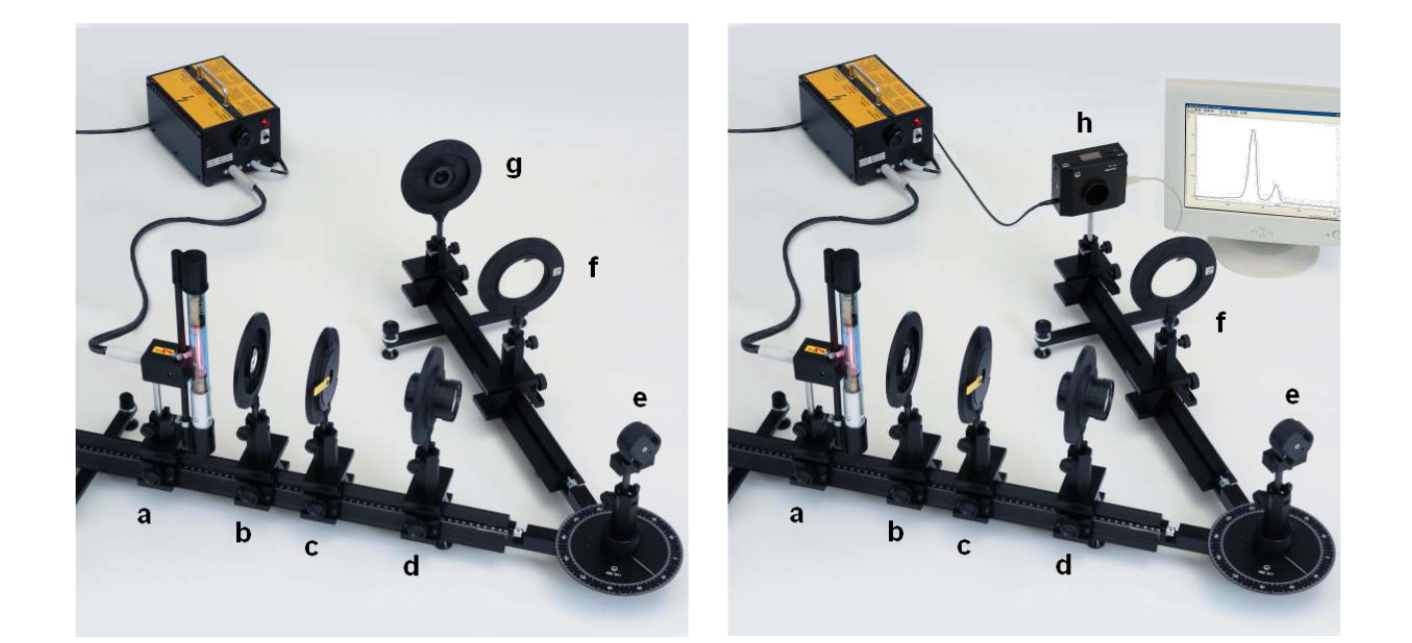
\includegraphics[width=0.7\linewidth]{figs/aufbau_balmer_serie.png}
    \caption{Versuchsaufbau mit Okular(links) und CCD-Kamera(rechts) \cite{praktikum}}
    \label{fig:balmeraufbau}
\end{figure}
Diese ist wie folgt aufgebaut: 

Es befindet sich eine Deuterium-Lampe (\textbf{a}), dessen Licht durch eine Sammellinese (\textbf{b}) mit Brennweite $f = 50mm$ auf ein verstellbareren Spalt (\textbf{c}) abgebildet wird, damit der einfallende Lichtstrahl begrenzt wird. 
Hinter dem Spalt befindet sich ein Projektionsobjektiv (\textbf{d}), mit Brennweite $f = 150mm$. 
Dieses soll genau im Abstand seiner Brennweite zum Spalt stehen, damit der Lichtstrahl parallel zum holographischen Gitter (\textbf{e}) einfällt. 
Dieses holographische Gitter ist ein Reflextrionsgitter welches sich auf der drehbaren Säule des Drehgelenk befindet und genutzt wird, um die Spektrallinien der Lampe aufzuspallten. 
Das reflektierte Licht wird anschliesend mit einer Sammellinse (\textbf{f}) der Brennweite $f=300mm$ auf einem Okular (\textbf{g}) abgebildet.
Das Okular kann alternativ mit einer CCD-Kamera (\textbf{h}) für genauere Messungen ersetzt werden.

\section{Durchfühung}

\paragraph{Justierung}

Um die Gitterkonstante zu bestimmen, müssen von einem bekannten Element die Spektrallinien untersucht werden. 
Dazu wird die Deutrium-Lampe (Balmer-Lampe) mit einer Quecksilder-Lampe (Hg-Lampe) ersätzt. 
Hierzu muss darauf geachtet werden das alle Bauteile des Aufbaus auf der gleichen Höhe bleiben, damit es keine Veränderungen der optischen Achse mit der Balmer-Lampe geben würde.
Es wird nun die Linse \textbf{b} so justiert, das ein scharfer Lichtfleck von der Lampe auf der Platte abgebildet wird.
Das Projektionsobjektiv \textbf{d} wird auf ungefähre Brennweite hinter dem Spalt positioniert. 
Es wird nun das Drehgelenk des Gitters (\textbf{e}) auf die 0$^\circ$ position gebracht und das Projektionobjektiv so verschoben, dass ein scharfes Bild der Lampe auf dem Spalt erkennbar ist, so wird der Spalt im Unendlichen abgebildet.
Zuletzt wird die Linse \textbf{f} so justiert, dass im Okular ein scharfes Bild des Spektrums zu erkennen ist. Dieses Bild soll eine beliebige Spektrallinie der ersten Ordnung sein.
Nun soll für den folgenden Versuchsteil die Winkel der optischen Bank ($\omega_B$) und der Winkel des Gitters ($\omega_G$) abgelesen werden.  
Damit diese werte benutzt werden können, müssen diese in die relevanten Winkel für das Gitter umgerechnet werden, siehe \cref{Gitter Balmer}. 
Mit Hilfe von \cref{Gitter Balmer} können die Winkel $\alpha$ und $\beta$ bestimmt werden: 
\begin{align}
    \alpha &= \omega_G \\  \beta &= \omega_B + \omega_G - 180^\circ 
    \label{Gitter Balmer}
\end{align}
wobei $\alpha$ der Einfallswinkel und $\beta$ der Ausfallswinkel ist.
Dieses Soll nach dem Austausch der Hg-Lampe und der Balmer-Lampe widerholt werden. 


\paragraph{Bestimmung der Gitterkonstante}

Die Gitterkonstante wird mit Hilfe der aufgenommen Spektrallinien der Hg-Lampe bestimmt.
Es wird nach der ersten Spektrallinie gesucht. 
Hierzu wird die Hellichkeit der Spektrallinien über den Spalt aufgedreht, wenn diese nicht sichtbar sind und dann auf etwa 1 Skalen Teil (0,1mm) eingestellt sind, aber so dass sie nicht verschinden.
Um zu vergleichen welche Wellenlänge gesehen werden, wird für die Auswertung die Hg-Linien von dem Anhang \cref{tab:Hg_lines} verwendet.
Es werden nun $\omega_B$ und $\omega_G$ abgelesen und mit \cref{tab:Hg_lines} zugeordnet.
Die Gitterkonstent wird mithilfe der Hg-Lampe bestimmt.
Es wird nach dem ersten Spektral linie gesucht, bis dies gefunden ist. 
Hier zu wird die hälichkeit der Spektrallinie über die Spalt aufgedreht, wenn diese nicht sichtbar sind und dann auf etwa 1 Skalen Teil (0,1mm) eingestellt, aber dass die nicht verschindet.
Um zu vergleichen welche Wellenlänge gesehen werden konnte für die auswertung wurde die Hg-Linien von dem Anhang \cref{tab:Hg_lines} zu nutzen.
Es werden nun $\omega_B$ und $\omega_G$ abgelesen und mit \cref{tab:Hg_lines} zugeordnet.


\paragraph{Untersuchung der Balmer-Linien}
Nach dem Tauschen der Lampen wird erstmal die Justierung widerholt. 
Nach der Justierung werden für jede Spektrallinie widerrum die Winkel $\omega_B$ und $\omega_G$ gemessen und der Abstand der Aufspaltung $d$ der Spektrallinien abgeschätzt.

\paragraph{Ersätzen Okular mit CCD-Kamera}
Es wird nun das Okular mit einer CCD-Kamera ersetzt, damit eine genauere Bestimmung der Spektrallinien stattfinden kann. 
Es wird ein Programm verwendet, welches die Intensität und Pixelkoordinate (Position der Intensität) aufnimmt und gegeneinander aufträgt. 
Falls die Intensität zu klein ist, kann im Programm die Schaltfläche vergrößert werden.
Das Programm gibt einen Winkel aus, den Ausfallswinkel, welches es aus den Pixelkoordinaten entnimmt: 
\begin{equation}
    \beta = \arctan(\frac{(1024-p)\cdot0,014mm}{f})
\end{equation}
wobei $p$ die Pixelkoordinate und $f$ die Brennweite der abbildenden Sammellinse sind.
Diese Linse wird noch verschoben, bis die Darstellung des Peaks scharf dargestellt werden kann (die Peaks sollen so dünn wie möglich sein).
Da die Intensität sehr empfindlich ist, wird mit Hilfe des Programms der Mittelwert der Intensitäten gebildet. 
Diese Werte werden gespeichert und die Winkel des Gitter aufgenommen. 
Es wird der gleiche Vorgang für die anderen Balmer-Linien durchgeführt.

\section{Bestimmung der Gitterkonstanten}
Um die Gitterkonstante zu berechnen wird die Gittergleichung für ein Reflexionsgitter genutzt:
\begin{equation}
  g\bigl(\sin\alpha + \sin\beta\bigr) = m\,\lambda
  \quad\Longrightarrow\quad
  g = \frac{m\,\lambda}{\sin\alpha + \sin\beta},
  \label{Gittergleichung}
\end{equation}
mit m die Ordnung, $\lambda$ die Wellenlänge, $\alpha$ der Einfallswinkel und $\beta$ der Ausfallswinkel, mit Fehler:
\begin{equation}
  \Delta g
  = \sqrt{
    \Bigl(\tfrac{\partial g}{\partial\alpha}\,\Delta\alpha\Bigr)^{2}
   +\Bigl(\tfrac{\partial g}{\partial\beta}\,\Delta\beta\Bigr)^{2}
  }.
  \label{Gitterfgleichung fehler}
\end{equation}
\begin{equation}
  \frac{\partial g}{\partial\theta_m}
  = \frac{m\,\lambda\,\cos\theta_m}{(\sin\theta_m + \sin\beta)^{2}},
  \quad
  \frac{\partial g}{\partial\beta}
  = \frac{m\,\lambda\,\cos\beta}{(\sin\theta_m + \sin\beta)^{2}}.
\end{equation}
\begin{equation}
    \Longrightarrow \Delta g = \sqrt{\Bigl(\tfrac{m\,\lambda\,\cos{\alpha}}{(\sin{\alpha}+\sin{\beta})^2}\,\Delta\alpha\Bigr)^2 + \Bigl(\frac{m\,\lambda\,\cos{\beta}}{(\sin{\alpha} + \sin{\beta})^2}\,\Delta\beta\Bigr)^2}.
\end{equation}

Es wird m = 1 gesetzt, da dies die Ordnung ist, die untersucht wird.
Die
 ausgerechneten Werte befinden sich in \cref{tab:gitterkonstante} mit den entsprechenden  Werten und dessen Fehler.
\begin{table}[htbp]
    \centering
    \begin{tabular}{|c|c|c|c|c|}
        Farbe & $\lambda$ / nm & $\alpha$ / ° & $\beta$ / ° & g / nm \\
        \hline 
        violett & 404,656 & 48,0 $\pm$ 0,5 & 13,0 $\pm$ 0,7 & 417,991 $\pm$ 8,757 \\
        violett & 407,783 & 49,0 $\pm$ 0,5 & 14,0 $\pm$ 0,7 & 409,161 $\pm$ 8,240 \\
        violett & 410,805 & 49,5 $\pm$ 0,5 & 14,5 $\pm$ 0,7 & 406,421 $\pm$ 8,026 \\
        violett & 433,922 & 50,5 $\pm$ 0,5 & 15,5 $\pm$ 0,7 & 417,689 $\pm$ 7,937 \\
        violett & 434,749 & 51,0 $\pm$ 0,5 & 16,0 $\pm$ 0,7 & 412,952 $\pm$ 7,699 \\
        blau & 435,833 & 51,0 $\pm$ 0,5 & 16,0 $\pm$ 0,7 & 413,981 $\pm$ 7,718 \\
        türkis & 491,607 & 55,5 $\pm$ 0,5 & 20,5 $\pm$ 0,7 & 418,626 $\pm$ 6,612 \\
        grün & 546,074 & 64,5 $\pm$ 0,3 & 24,5 $\pm$ 0,5 & 415,067 $\pm$ 3,681 \\
        gelb & 576,960 & 67,5 $\pm$ 0,3 & 27,5 $\pm$ 0,5 & 416,952 $\pm$ 3,330 \\
        gelb & 579,066 & 68,0 $\pm$ 0,3 & 28,0 $\pm$ 0,5 & 415,176 $\pm$ 3,258 \\
        rot & 623,440 & 65,0 $\pm$ 0,3 & 35,0 $\pm$ 0,5 & 421,428 $\pm$ 3,077 \\
        rot & 671,643 & 61.5 $\pm$ 0,5 & 36.5 $\pm$ 0,7 & 455.771 $\pm$ 4.890 \\
        rot & 690,752 & 62.5 $\pm$ 0,5 & 37.5 $\pm$ 0,7 & 461.803 $\pm$ 4.782 
    \end{tabular}
    \caption{Berechnete Gitterkonstante und dessen Fehler}
    \label{tab:gitterkonstante}
\end{table}
Es ist zu bemerken, dass die roten Spektrallinien für $\omega_B = 145^\circ$ nicht sichtbar waren. $\omega_B$ wurde zur Überprüfung geändert, und die Spektrallinien nochmal ausfgenommen. 
Zu beachten ist, dass diese Werte nicht genau übereinstimmen, was mit schlechtem abschätzen zu tun haben könnte, da zum Beispiel $61,2^\circ$ und $61,0^\circ$ kaum zu unterscheiden waren.
Mit der Erkenntnis dieser Fehlerquelle sind die Werte angemessen.
Zusätzlich waren manche Linien so blass, das diese kaum erkannt wurden und mehr Linien beobachtet wurden. 
Diese wurden aber nicht aufgenommen, da diese sehr schlecht zu sehen waren. 
Um einen festen Wert für die Berechnung der Balmer-Linien zu haben , wurde der Mittelwert von den ausgerechneten Gitterkonstanten genommen:

\begin{equation}
  \overline{g}
  = \frac{\sum_{i=1}^{N} \bigl(g_i/\Delta g_i\bigr)}
         {\sum_{i=1}^{N} \bigl(1/\Delta g_i\bigr)},
  \quad
  \Delta\overline{g}
  = \sqrt{\frac{N}{\sum_{i=1}^{N} 1/(\Delta g_i)^{2}}}\,.
\end{equation}

Es ergibt sich nun die Gitterkonstante:
\begin{equation}
    \overline{g} = (420.76 \pm 1.51) nm.
    \label{gitterkon}
\end{equation}
Dieser Wert passt nicht zu allen g-Werten, aber da die Meisten Werte übereinstimmen, ist es somit ein sinvoller Wert. 

\section{Bestimmung der Balmerlinien} \label{Bestimmung der Balmer}

Mit der Gitterkonstante können nun die Wellenlängen der Balmer-Lampe berechnet werden. 
Dies kann durch die Gittergleichung \ref{Gittergleichung} in der ersten Ordnung berechnet werden.
Die dazu gehörige Wellenlängen sind zwischen 388nm und 656nm sichtbar~\cite{Ulm} und werden zu den Messungen zugeordnet.
Die Emissionslinien sind dabei die Übergänge von Energieniveaus $n > 2 \xrightarrow{} n = 2$ 
Die Photonen die den Übergang beschreiben, können durch die Rydberg-Formel (\cite{Demtröder_Ex3}, S.100) 
\begin{equation}
  \frac{1}{\lambda}
  = Ry\Bigl(\tfrac{1}{2^{2}} - \tfrac{1}{n^{2}}\Bigr),
  \quad n=3,4,5,\dots
  \label{Rydberg-Formel}
\end{equation}
berechnet werden.
Diese werden noch im \cref{Rydberg-konst} bestimmt. 
Es werden nochmals die Winkel für die bestimmten Emissionslinien aufgenommen und die ausgerechneten Werte in \cref{tab: gesehenes deut}, so wie deren Literaturwert, aufgelistet. 

Wärend des Versuches wurden nur 3 Emissionslinien beobachtet, dies könnte an der fehlenden Abschirmung der Lampe liegen, welche durch Reflexion an der linse vor dem Okular, die schwer zu sehenden Emissionslinien, überleuchtet hat. %Versuche zu sagen, dass wegen das licht der lampe die linie nicht zu sehen ist.
Diese könnten zu H$_\alpha$, H$_\beta$ und H$_\gamma$ zugeordnet werden.

\begin{table}[htbp]
    \centering
    \begin{tabular}{|c|c|c|c|}
        Linie & d / Skt & $\Delta \beta$ /$10^{-2}$ rad & $\Delta \lambda$ /nm \\
        \hline
        $H_\alpha$ & 0,5 $\pm$ 0,1 & 46,36 $\pm$ 3,33 & 156,82 $\pm$ 54,97 \\
        $H_\beta$ & 1,0 $\pm$ 0,1 & 32,17 $\pm$ 3,33 & 126,81 $\pm$ 20,14 \\
        $H_\gamma$ & 1,5 $\pm$ 0,1 & 16,51 $\pm$ 3,33 & 66,80 $\pm$ 13,85 \\


    \end{tabular}
    \caption{Gesehenes Deuterium}
    \label{tab: gesehenes deut}
\end{table}

Es ist zu sehen, dass die berechneten Wellenlängen nicht mit dem Literaturwert übereinstimmen. 
Dies könnte an der Näherung der Winkel liegen, da diese zum Beispiel als $55,3^\circ \approx 55,5^\circ$ festgehalten wurden.
Zusätzlich hätten die Fehler auch zu klein Geschetzt werden können.
Obwohl die Werte innerhalb ihrer Fehler nicht mit den Literaturwerten übereinstimmen, sind die Werte genau genug, um zugeordnet zu werden. 


\subsection{Bestimmung der Isotopieaufspaltung}

Bei der Unteruchung der Emissionslinien der Balmer-linien, wurde gesehen, dass die Emissionslinien eine zweite Emissionslinie existiert.
Der Grund hierfür ist, dass die Balmer-Lampe nicht rein aus Deuterium, sonder auch aus Wasserstoff besteht, im Verhältnis von $\approx 1 : 2$ (\cite{praktikum}). 
Dies weist darauf hin, das die Kermasse einen Einfluss auf die Energieniveaus hat. 
Aus der Quantenmechanik kann die Rydberg-Konstante zusätzlich mit 
\begin{equation}
  R_{\mathrm{y}} = \frac{\mu\,e^4}{8\,c\,\epsilon_0^2\,h^3}
\end{equation}
beschrieben werden(\cite{Demtröder_Ex3}, S.101). Dabei ist zu beachten, dass dieser wert von der reduzierten Masse abhängt:
\begin{equation}
    \mu = \frac{m_e \cdot m_K}{m_e + m_K} = \frac{m_e}{1+\frac{m_e}{m_K}},
\end{equation}
mit $m_e$ die Elektronen Masse und die Kernmasse $m_K$.
Somit kann eine feste Rydbergkonstante ($Ry_\infty$) bestimmt werden: 
\begin{equation}
    Ry = \frac{1}{1+\frac{m_e}{m_K}}\cdot \frac{\mu m_e e^4}{8c \epsilon_0^2h^3} = \frac{1}{1 + \frac{m_e}{m_K}}\cdot Ry_\infty.
\end{equation}
Da das Deuterium ein extra Neutron hat, ist dieses schwerer, und somit ist die Rydberg-Konstante kleiner und so auch proportional zur Wellenlänge. 
Dieses wurde auch für größere Wellenlänge deutlicher sichtbar.
Diese Aufspaltung wird als Isotopieaufspaltung bezeichnet, wobei es sich in diesem fall über ein Masseneffekt der Isotopiaufspaltung handelt.

Mit der Skala im Okular kann die Breite d der Isotopieaufspaltung für die Emissionslinien geschätzt werden. 
Diese befinden sich in \cref{tab:H_D_lines}.

Mit \cref{Gittergleichung}
\begin{equation}
  \lambda = g\,(\sin\alpha + \sin\beta),
  \quad
\frac{\Delta\lambda}{\Delta\beta} \approx 
  \frac{\partial\lambda}{\partial\beta} = g\,\cos\beta,
  \label{deltalambda}
  \quad
  \Delta\beta \approx \frac{d}{f},
\end{equation}
und mit der Brennweite der Abbildungslinse lässt sich der Winkel $\Delta\beta$ mit 
\begin{equation}
    \Delta\beta = \arctan\Bigl(\frac{d}{f}\Bigr) \approx \frac{d}{f} \quad \text{für } d \ll f
\end{equation}
berechnen lassen.

Diese Werte sind aber ungenau, da die Aufspaltung sehr schwer zu erkennen war und nur mit Mühe abgeschätzt wurde.

Die CCD-Kamera hat dieses Problem aber nicht und kann die Isotopieaufspaltung genauer messen.

Die gemessenen Intensitäten bilden Peaks die in \cref{fig:H_a}, \cref{fig:H_b} und \cref{fig:H_g} dargestellt sind. 
\begin{figure}
    \centering
    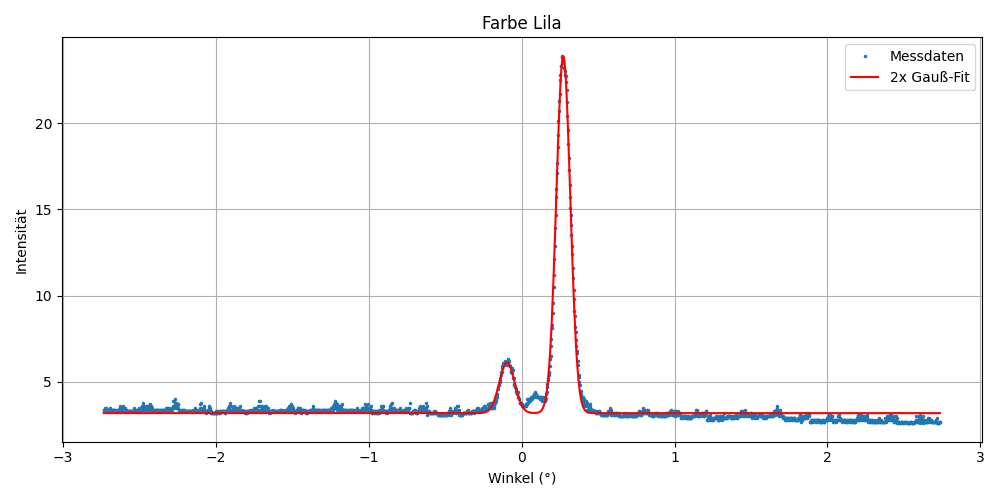
\includegraphics[width=\linewidth]{figs/dt_lila_145_51_5.png}
    \caption{Isotopieaufspaltung von der $H_{\gamma}$ mit $\chi_{red} = 0.09$}
    \label{fig:H_g}
\end{figure}

Hierbei sind mehrere Peaks zu erkennen und können durch folgende Gauß-Funktion 
\begin{equation}
    I(\beta) = \sum_i^2 A_i \cdot \exp{\Bigl(-\frac{\beta-\mu_i}{2\sigma_i}}\Bigr) +b
\end{equation}
gefittet werden, wobei b der Offset ist und $\beta$ der Winkel. 

Die berechneten Werte sind in \cref{tab:Peaks} zu sehen.
Die Isotopieaufspaltung wird durch 
$\Delta\beta = |\mu_2 - \mu_1|$
gegeben. 
Man erhält:
\begin{table}[htbp]
    \centering
    \begin{tabular}{|c|c|c|c|c|}
        Linie & $\alpha$ / ° & $\beta$ / ° & $\Delta\beta$ / ° & $\Delta\lambda$ / nm \\
        \hline
        $H_\alpha$& 62,0 & 37,0 & 0,167 $\pm$ 0,003 & 0,980 $\pm$ 0,739 \\
        $H_\beta$ & 55,5 & 20,5 & 0,047 $\pm$ 0,003 & 0,322 $\pm$ 0,122 \\
        $H_\gamma$ & 51,5 & 16,5 & 0,368 $\pm$ 0,001 & 2,587 $\pm$ 0,766 \\
        $H_\delta$ & 49,0 & 14,0 & 1,694 $\pm$ 0,085 & 12,052 $\pm$ 3,066 \\
    \end{tabular}
    \caption{Isotopiaufspaltung der Balmer-Lampe anhand der CCD-Kamera}
    \label{tab:Isotopiaufspaltung}
\end{table}
Obwohl nur 3 Emissionslinien gesehen wurden, hat die CCD- Kamera noch eine zusätzlich aufgenommen, welches als $H_\delta$ vermutet wird.
Die berechneten Werte weichen aber signifikant ab.
Dies lag vermutlich daran, dass die Balmer-Lampe nicht abgeschirmt war und somit die Genauigkeit der Messung beeinträchtigt hat. 
Es kann aber trotzdem die Aufspaltung beobachten und somit wurde das Ziel der Untersuchung erreicht.

\subsection{Bestimmung der Rydberg-Konstante und des Plankschen Wirkungsquantum}
\paragraph{Rydberg-Konstante} \label{Rydberg-konst}
Wie schon in Abschnitt \ref{Bestimmung der Balmer} erwähnt kann die Rydberg-Konstante über die Wellenlänge bestimmt werden.
Dafür ist eine folgende Umrechnung nötig:
\begin{equation}
  Ry
  = \frac{1/\lambda}{\bigl(\tfrac{1}{4} - \tfrac{1}{n^{2}}\bigr)},
  \quad
  \Delta Ry
  = \frac{\Delta\lambda}{\lambda^{2}\,\bigl(\tfrac{1}{4} - \tfrac{1}{n^{2}}\bigr)}.
\end{equation}
Mit den berechneten Werten in \cref{tab:Rydberg} sieht man, dass die Werte miteinander übereinstimmen, aber unterschiedliche Wert haben. 

\begin{table}[htbp]
    \centering
    \begin{tabular}{|c|c|c|c|}
        Linie & $\lambda$ / nm & n & Rydberg-Konstante /$10^7$ m \\
        \hline
        $H_\alpha$ & 620,049 $\pm$ 4,091 & 5 & 1,161 $\pm$ 0,008 \\
        $H_\beta$ & 494,113 $\pm$ 4,393 & 4 & 1,079 $\pm$ 0,010  \\
        $H_\gamma$ & 442,969 $\pm$ 4,508 & 3 & 1,075 $\pm$ 0,011 \\
    \end{tabular}
    \caption{Berechneten Rydbergkonstanten für die berechentn Wellenlängen}
    \label{tab:Rydberg}
\end{table}

Um den Wert zu bestimmen wird das gleiche Verfahren wie bei der Gitterkonstante benutzt:
\begin{equation}
  \overline{g}
  = \frac{\sum_{i=1}^{N} \bigl(g_i/\Delta g_i\bigr)}
         {\sum_{i=1}^{N} \bigl(1/\Delta g_i\bigr)},
  \quad
  \Delta\overline{g}
  = \sqrt{\frac{N}{\sum_{i=1}^{N} 1/(\Delta g_i)^{2}}}\,.
\end{equation}
Dies liefert einen Wert von:
\begin{equation}
    Ry = (1,105 \pm 0,006)\cdot 10^7 \frac{1}{m}.
\end{equation}
Dieser Wert stimmt sehr gut mit dem Literatur Wert (\cite{Demtröder_Ex3}, S.101) von der Rydbergkonstante welches 
\begin{align}
    Ry_{lit} = 1,097 \frac{1}{m} ist,
\end{align}
in einer $2\sigma$-Umgebung vom experimentellen Wert liegt.
Es könnte auch einen Felher in der Fehlerrechnung vorgekommen sein, da dieser sehr klein ist.

\paragraph{Planksche Wirkungsquantum}

Mit Hilfe der berechneten Rydberg-Konstante kann das Planksche-Wirkungsquantum bestimmt werden:

\begin{equation}
    Ry = \frac{\mu e^4}{8 c \epsilon_0^2h^3}
\end{equation}
\begin{equation}
  \Leftrightarrow h
  = \Bigl(\tfrac{m_e\,e^{4}}{8\,\varepsilon_{0}^{2}\,c\,Ry}\Bigr)^{1/3},
  \quad
  \Delta h
  = \frac{1}{3}
    \Bigl(\tfrac{m_e\,e^{4}}{8\,\varepsilon_{0}^{2}\,c}\Bigr)^{1/3}
    Ry^{-4/3}\,\Delta Ry.
\end{equation}

Somit wird das Planksche-Wirkungsquantum bestimmt auf:
\begin{equation}
    h = (6.61 \pm 0.11)\cdot 10^{-34} J\cdots
\end{equation}
berechent was mit dem Literaturwert (\cite{Demtröder_Ex3}, S.75) von
\begin{equation}
    h = 6,63 \cdot10^{-34} J\cdot s
\end{equation}
sehr gut übereinstimmt.
Dieser liegt auch innerhalb einer $2\sigma$-Umgebung des experimentellen Wertes und und stimmt mit der Berechnung des Plankschen-Wirkungsquantum durch den Photoeffekt überein.


\section{Weitergehende Überlegungen}
\subsection{Möglicher Ursprung der anderen auftrennen Spektrallinien}
In diesem Versuchsteil werden aber nicht nur die Balmer-Linien beobachtet. 
Durch einfallendes Licht von anderen Quellen, vor allem elektronische Geräte die für die Messung verwendet werden, besteht die Möglichkeit, dass dieses auch aufgenommen wird.
Sehr wichtig ist, dass der EffeKt des Streulichtes berücksichtigt wird, welches die Bamler-Lampe emittiert, da dieses anders reflektiert werden kann, als wenn es mittig auf dem Gitter trifft.
Wenn die Linsen beschädigt wäre, dann würden zusätzlich Linsenfehler oder Aberrationen auftreten und diese müssen somit auch berücksichtigt werden. 
Zusätzlich muss beachtet werden, dass es mehr als eine Ordnung gibt und somit die letzten beobatbaren Linien der Ordnung mit Linien einer höheren Ordnung überschneiden kann.

\subsection{Doppler-Verbreitung}

Wegen der Termischen Bewegung der Atome relative zu einem ruhenden Betrachter, entsteht eine Doppler-Verschiebung des emitierten Photonen. 
Dies führ zu einer verbreiterung der Spektrallinien über ihre natürliche Breite hinaus, welche mit der Formel (\cite{Demtröder_Ex3}, S.230)
\begin{equation}
    \delta\lambda = \frac{\lambda_0}{c}\cdot \sqrt{\frac{8k_BT\cdot ln2}{m}}
\end{equation}
beschrieben werden kann.
Dabei ist $\delta\lambda$ die Halbwertsbreite, die Temperatur $T \approx 1000K$ (\cite{praktikum}) und m die masse des Atomes (2$m_H \approx m_D$)
Diese Werte werden in \cref{tab:dopplerTemp}
\begin{table}[htbp]
    \centering
    \begin{tabular}{|c|c|c|c|}
    \hline
    Linie & Literaturwert $\lambda$ in nm & $\delta\lambda$ für $^1H$ in nm & $\delta\lambda$ für $^2H$ in nm \\
    \midrule
    H$_\alpha$ & 656,28 & 0,015 & 0,011 \\
    H$_\beta$ & 486,13 & 0,011 & 0,008 \\
    H$_\gamma$  & 434,05 & 0,010 & 0,007 \\
    \hline
    \end{tabular}
    \caption{(Theoretische) Doppler-Verbreitung von Wasserstoff und Deuterium}
    \label{tab:dopplerTemp}
\end{table}

Um die natürliche Linienbreite $\delta\nu$ zu berechnen, wird die Formel
\begin{equation}
    \delta \nu = \frac{1}{2\pi \cdot \tau}
\end{equation}
benutzt (\cite{Demtröder_Ex3}, S.228f), mit $\tau$ die Lebesdauer. 
Diese Formel hängt nur von extakten Werten ab und die Linienbreite kann auch von der Heisenberg'schen Unschärferelation hergeleitet werden.  
Die Lebesdauer von Atomen liegt in der Größenordnung von $10^{-8}s$. 
Dies führt dazu, dass $\delta\nu$ in der größenordnung von $16MHz$  ist und durch $\frac{\Delta\nu}{\nu} = \frac{\Delta\lambda}{\lambda}$ mit $\nu = \frac{c}{\lambda}$ führt dazu, dass die Linienbreit in der Ordnung von $10^{-14}nm$ ist und somit vernachlässigbar groß gegenüber der Dopplerverbreitung ist.
Daher ist es sinvoller die Doppler-Verbreitung mit den Hablwertsbreiten der berechneten Gaußkurven zu vergleichen.
Diese kann bestimmt man mit:
\begin{equation}
    \delta\beta = 2\sqrt{\ln{2}}\cdot \sigma,
\end{equation}
wobei $\sigma$ die Halbwertsbrete ist.
Hierdurch kann man mit \cref{deltalambda} die Wellenlängendifferenz berechnen.
Die berechneten Werte sind in \cref{tab:gemhalb}.

\begin{table}[htbp]
    \centering
    \begin{tabular}{|c|c|c|}
    Linie & $\delta\lambda$ für $^1$H in nm & $\delta\lambda$ für $^2$H in nm \\
    \hline
        H$_\alpha$ & 0.848 ± 0.006 & 0.586 ± 0.049 nm \\
        H$_\beta$ & 2.258 ± 0.051 nm & 0.609 ± 0.003 \\
        H$_\gamma$ & 0.831 ± 0.021 nm & 0.758 ± 0.004 nm
    \end{tabular}
    \caption{Gemessene Halbwertsbreite für bekannte Spektrallinien}
    \label{tab:gemhalb}
\end{table}
Es ist deutlich zu sehen, dass die Halbwertsbreiten sehr groß sind. 
Die Fehler sind auch sehr klein, dies kann an einer falschen Anpassung einiger Gaußkurven ( zum Beispiel bei H$_\beta$ konnte die Gauß Kurve nicht gut zu dem zeiten Peak angepasst werden ) liegen.
Zusätzlich hätte der Breite der Peaks beim messen besser eingestellt werden können, da der Aufbau möglicherweise nicht richtig justiert wurde, sodass die Spaltbreite zu groß gewählt wurde und nicht vollständig ausgeleuchtet war oder ,sodass das Streulicht die Basisintensität durch fehlender Abschirmung angehoben hat und dadurch die Peaks "flacher" erschienen.


\subsection{Auflösevermögen des Gitters}

Anschliessend wird das Auflösungsvermögen des Gitters abgeschätzt. 
Dies wird mit der Formel 
\begin{equation}
    A = \frac{\lambda}{\Delta\lambda} = m \cdot N
\end{equation}
gemacht, wobei m die Ordnungs Zahl ist und N die Anzahl der Beleichteten Spalten. 
Das gesammte Gitter beträgt eine 25 mm x 25 mm Fläche:
\begin{equation}
    \Rightarrow N = \frac{d}{g}, d = 25mm
\end{equation}
\begin{equation}
    \Rightarrow A = \frac{25mm}{420,76nm} = (5,94 \pm 0,02) \cdot 10^4
\end{equation}
So wäre es möglich alle Aufspaltungen zu messen, da das Auflösungsvermögen vom Gitter so groß ist. 
Dies würde aber bedeuten, dass das ganze Gitter beleuchtet werden müsste, welches aber bei der Untersuchung der Isotopieaufspaltung stören würde, da dies nicht mehr sichtbar wäre.
Um dieses wiederum messen zu können, müsste der Spalt verringert werden und somit auch das Licht welches auf dem Gitter fällt.
